%******* ME ME ME!!!

%As will be discussed further in the following chapter, the ultimate realisation of a parallel reality system may in fact be one in which a mix of RW and VR visuals are presented in a manner more similar to familiar AR systems, but maintaining the ability to view either complete environment individually at the total exclusion of the other.

%=========================================================================================================

\begin{quote}
	\textit{``If the chaos of the nineties reflects a radical shift in the paradigms of visual literacy, the final shift away from the Lascaux/Gutenberg tradition of a pre-holographic society, what should we expect from this newer technology, with his promise of discrete encoding and subsequent reconstruction of the full range of sensory perception?''}
\end{quote}
\hfill \textit{Burning Chrome, William Gibson}
\\
\\

%=========================================================================================================

\label{chapter-conclusions}

Alternate realities have fascinated mankind since early prehistory and with the advent of the computer and the smartphone we have seen the rise of many different categories of alternate reality that seek to replace, augment, diminish and mix with our familiar real world to expand our capabilities and our understanding. This thesis has introduced parallel reality as a new category of alternate reality comprising two environments that the user may freely switch between, one real and the other virtual, both complete unto themselves. The benefits that such a system imparts upon the user by granting them the ability to mitigate the extended vacancy problem and explore parallel real and virtual environments in tandem have been shown through the development of the Mirrorshades parallel reality platform and its application to user studies within the realm of cultural heritage. Evaluation of these studies has lead to the establishment of a number of best practices for future parallel reality endeavours.

\begin{figure}[t]
	\begin{center}
		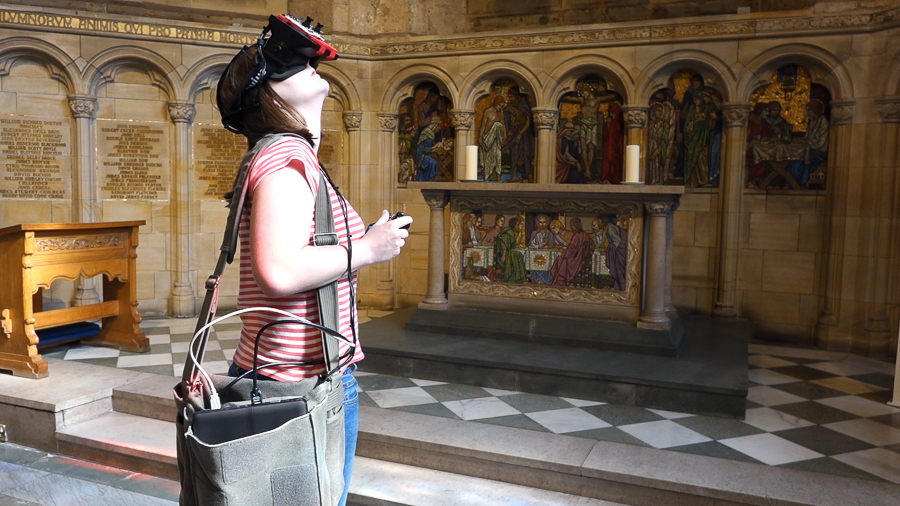
\includegraphics[width=\textwidth]{participant-f-4.jpg}
		\caption{The Mirrorshades parallel reality platform in use at a 15th century chapel.}
		\label{participant-f-4.jpg}
	\end{center}	
\end{figure}

\begin{figure}[t]
	\begin{center}
		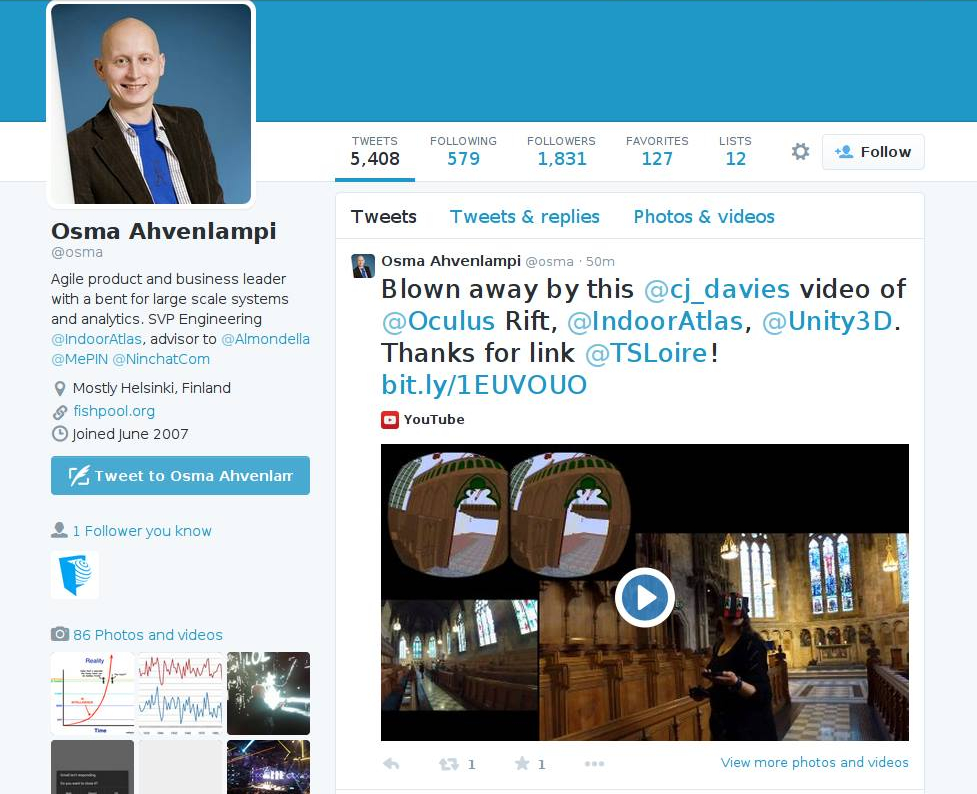
\includegraphics[width=0.8\textwidth]{osma-twitter.jpg}
		\caption{Praise for the Mirrorshades parallel reality platform from IndoorAtlas' senior vice president of engineering.}
		\label{osma-twitter.jpg}
	\end{center}	
\end{figure}

%=========================================================================================================

\section{Contributions}

As listed in section \ref{intro-contributions} the contributions of this thesis can be summarized at a high level as follows:

\begin{itemize}
	\item The introduction of parallel reality as a new category of alternate reality that allows users to experience complete real and virtual environments in tandem and represents an avenue for further mitigation of the vacancy problem.
	\item The framing of parallel reality through a thorough investigation and extension of previous taxonomies that classify and distinguish between alternate reality terminology.
	\item The introduction of the combined Milgram/Waterworth model for visualising alternate reality experiences, including those of parallel reality systems.
	\item The visualisation of the vacancy problem upon the combined Milgram/Waterworth model, leading to the definition of the extended vacancy problem.
	\item Development of a preliminary parallel reality platform, the Virtual Time Window, through extension of the Second Life client.
	\item Development of a second parallel reality platform, dubbed Mirrorshades, that uses the Unity game engine to combine new virtual reality hardware with novel indoor positioning technology.
	\item Evaluation of the Mirrorshades platform through user studies of a real world use case study within the realm of virtual heritage, including the discussion and application of an established presence questionnaire to a parallel reality experience.
	\item Creation and discussion of a set of best practices for future parallel reality endeavours.
\end{itemize}

%=========================================================================================================

\section{Discussion}

%=========================================================================================================

\subsection{Objectives}

In reference to the objectives as listed in section \ref{objectivesandmethodology} and reproduced here for discussion, this thesis has met what it set out to.

\begin{enumerate}
	\item[1] Introduce the parallel reality concept by situating it within the larger ecosystem of existing categories of alternate reality, through a thorough exploration of existing alternate reality definitions, taxonomies and frameworks, performing updates, modifications and extensions where required.
\end{enumerate}

The introduction of parallel reality, in a clear and unambiguous fashion, as a new category of alternate reality was no simple task, as decades of research into alternate realities has furnished us with a rich continuum of approaches and technologies for creating, combining, augmenting and diminishing real and virtual environments. The fact that there are often no clear boundaries between where one category ends and another begins, with continuums being more popular than discrete categorisation, due largely to the inherently subjective nature of space experience, has lead to many common labels applying to multiple different scenarios. Whilst some of these are compatible if not identical, some are almost contradictory. However it is seldom the case that any use of the terms in the literature is genuinely incorrect.

Thus the purpose of the extensive review in chapter \ref{chapter-background} of existing techniques for categorising and distinguishing between different alternate realities was to ensure that parallel reality was introduced in a fashion that made its place in comparison to all the other alternate reality terms clear and unambiguous.

It is important to appreciate that much of it is subjective however. Lots of abstract thought had to go into this, verging on the philosophical in places but always trying to ground it in science.

\begin{enumerate}
	\item[2] Develop a suitable model for the illustration of experience in parallel reality scenarios, allowing not only for comparison and contrast between parallel reality and other alternate reality experiences, but also for illustration of different implementations of parallel reality experience.
\end{enumerate}

As one of the direct products of the work discussed for objective 1, the combined Milgram/Waterworth model was produced for this purpose and represents an indispensable tool for visualising, discussing and comparing alternate reality experiences. By combining the relatively objective assessment of where the percepts a user is perceiving originate from (the Milgram and Kishino approach) with the more subjective and experiential assessment of the direction and magnitude of human attention (the Waterworth and Waterworth approach) we are gifted the ability to assess both vantages onto an alternate reality experience and to more easily relate them and see any relationships.

One of these relationships that becomes apparent when considering the two original models combined in the manner of the combined Milgram/Waterworth model is that of how the vacancy problem, as identified by Lifton, can be explained in a more scientific fashion in reference both to the Milgram and Kishino model and to the Waterworth and Waterworth model, leading to the introduction of the definition of the extended vacancy problem.

\begin{enumerate}
	\item[3] Develop a parallel reality system suitable for deployment to real world user studies to effect comparison against previous categories of alternate reality.
\end{enumerate}

Initially it was thought that a rewarding parallel reality experience might be possible through leveraging an existing modality of alternate reality interaction, that of Situated Simulation (SitSim). The VTW project discussed in chapter \ref{chapter-vtw} investigated this possibility.

Two major things wrong with it.

Firstly the modality of interaction did not encapsulate the style of interaction originally envisaged of the parallel reality concept, that of wholly switching between discrete real and virtual environments, due to the way in which the virtual was always seen as a small window surrounded by the larger and all encompassing real.

When SitSim was considered as a possible avenue through which parallel reality could manifest, the focus was upon the environmental aspect. It was not until testing the platform at St Andrews Cathedral that the importance of the experiential aspect become clear. This led to the explicit realisation and appreciation of these two aspects of the parallel reality concept, both of which needed to be realised in order for parallel reality to manifest in its originally envisaged splendour (see discussion in section \ref{real-world-experience-of-vtw}).

The performance of the VTW platform was also somewhat lacklustre, which limited its utility even ignoring the wrong modality. The decision to make use of the Second Life/OpenSim software environment, in order to make use of existing virtual content without having to embark upon a lengthy conversion process, limited the choice of tablet upon which the platform could operate to the very small number (at the time) of x86 tablet computers. None of these had the graphical performance of today's popular Android and iOS tablets and this combined with the fact that Second Life/OpenSim is not in any way optimised nor designed for mobile use and is slower even than other non mobile 3D engines due to the ephemeral nature of its content meant that graphical performance and quality were low.

The low performance and poor accessibility of the tablet's GPS and orientation sensing hardware also meant that a lengthy process of hardware prototyping and integration was required, and due to the limited control interfaces provided by the Second Life client it was necessary to embark upon a lengthy software development stage that went as far as to add serial I/O to the client.


The development and evaluation of the VTW platform highlighted the importance of the experiential aspect of parallel reality, as well as providing insight into performance requirements and best practices over what software/hardware environment to make use of. And all of this led to the creation of the Mirrorshades platform.

While the physical manifestation of the Mirrorshades platform is far less convenient and far more `research equipment' than VTW, due to the fact that it fills a satchel that must be worn by the user and also occupies both of their hands with equipment, it fully realised the envisaged experience of parallel reality and did so with higher graphical performance and quality along with higher orientation and position tracking quality thanks to the adoption of a more suitable software environment coupled with a new stereoscopic 3D HMD.


\begin{enumerate}	
	\item[4] Identify and put into practice suitable assessment techniques to ascertain the merit of parallel reality in relation to previous categories of alternate reality.
\end{enumerate}

Here once again the inherently subjective nature of real and virtual space experience make such an assessment difficult. However with the utility of the combined Milgram/Waterworth model and the extended vacancy problem definition, a combination of both qualitative and quantitative results led to a number of interesting observations and discoveries.

subjective and presence

The novel nature of a parallel reality experience, promoting the interaction with two discrete environments rather than with one mixed environment or only a virtual environment at the complete suppression of the real environment, led to an interesting challenge where no widely adopted presence questionnaire could be directly applied to the experiences. However by realising that the categorical design of the igroup presence questionnaire allowed the different aspect of a parallel reality system to be separated from more traditional VR experiences allowed it to be applied to this new category of alternate reality and served to reinforce with more quantitative values what was being observed in qualitative feedback.
	
\begin{enumerate}
	\item[5] Identify aspects of the implementation of a parallel reality system that positively or negatively effect the user experience, along with assessment methodologies to ascertain these effects, putting these into practice within real world user studies.
\end{enumerate}

\begin{enumerate}
	\item[6] Evaluate user studies to inform creation of best practise recommendations for future parallel reality endeavours.
\end{enumerate}





Critical analysis of the consequences and impact of the research

Broader set of findings

Talk about the lot of hitherto unknown facts and preferences that have now been revealed




%=========================================================================================================

\subsection{Shortcomings}

%=========================================================================================================

\subsection{Emergent Preferences Toward AR Style Mix}

Looking back to the intro of chapter 1

This is not an augmented reality system which superimposes virtual objects upon the real
world.

emphasis is on objects and their individual nature, vs the entire virtual environment of a parallel reality system




and in section 2.4 where we said

In this regard we further distinguish a parallel reality system from an augmented
reality system by defining the former as allowing its user to switch between two different primary
environments whereas the latter augments one particular primary environment.



the mix came out on top and is experientially very similar to AR

considering 3.7.5

environmental aspect vs experiential aspect

this mixed parallel reality is distinct to AR in terms of the environmental aspect, but not really in terms of the experiential aspect
	except that by having this distinction in the environmental aspect, a system that adopts this mix that seems like AR also has the ability to present the distinct experiential aspect by \textbf{also} allowing the user to transition wholly to one environment at the complete exclusion of the other

%=========================================================================================================

\section{Future Work}

The introduction of parallel reality in this thesis along with the evaluation of its first involved implementations, which investigated leveraging an existing modality of alternate reality interaction with VTW and explored a novel new style of alternate reality interaction with Mirrorshades, is only the beginning of an extended course of study that will be required to fully understand and come to appreciate the benefits that it can provide as a concept. The following discussion highlights but a few choice avenues that the future investigation of parallel reality would do well to explore and should by no means be considered an exhaustive list of possible sources of extension; after all the \textit{``potential applications of VR are really only limited by the imaginations of talented individuals''}~\cite{Giuseppe2014a}. Since its recent rejuvenation at the hands of Oculus, the field of virtual reality has seen its rate of progress and advancement massively accelerated. With this in mind, the potential of these avenues of further investigation into the parallel reality concept to produce fruitful results is substantial.

Most evident is the matter of hardware. The Mirrorshades parallel reality platform used in the user studies presented in this thesis is a somewhat cumbersome package of HMD, laptop, battery pack, smartphone, games console controller and myriad cables, occupying both of the user's hands and requiring them to carry a satchel of not insubstantial size and weight (large enough for an 11`` laptop and around 2.5kg in total). To posit that the cumbersome nature of the platform had a directly detrimental effect upon the quality of experience received by the participants is no stretch of the imagination and improvements in this regard will be required for parallel reality to see deployment and use in anything but controlled laboratory or user study conditions. As discussed in section \ref{mobile-client} we are already beginning to see the advent of hardware platforms that present a much improved basis for parallel reality experiences. A platform such as Samsung Gear VR, perhaps modified with stereoscopic video see-through abilities, would represent a fully contained single unit parallel reality experience, suitable for handing to a user in the same manner that audio guides are given out at many of the world's museums. Google's Cardboard platform\footnote{\url{https://www.google.com/get/cardboard/}} also presents an intriguing possibility for future parallel reality implementations at very low cost, making use of nothing more than a folded piece of cardboard and two plastic lenses combined with any of a wide variety of smartphones to form a rudimentary HMD which users could bring to their eyes to perform a transition into VR and remove when they wish to view their real surroundings. Furthermore, improvements to the performance of the platforms, in terms of the visual acuity of both real and virtual content as well as the accuracy of the positioning and registration, will present beneficial results both to casual users and to experts wishing to use such a modality of interaction for serious study. 

Investigating the application of parallel reality to other domains represents possibly the largest avenue of potential extension. While the user studies discussed in this thesis experimentally demonstrated the worth of parallel reality when applied to the field of cultural heritage, parallel reality as a concept can be applied to many fields. Postulating for but a moment one can imagine how parallel reality could be applied to architecture to allow people to walk through a house as it is still being built or renovated and switch to seeing its destined form, to using the physical layout of an environment as a canvas for novel artistic expression, to the study of polysocial interactions involving real and VR parties, to new styles of gaming that merge both real and virtual play fields, to allowing rescue workers to study the state of a building before a fire broke out and identify dangers that could now be hidden in the flames. As society becomes both more familiar with and more dependent upon almost constant connection to the virtual, whether in the form of 2D Web based social networks and apps or richer multimedia experiences, the utility of platforms that allow real and virtual environments to be cycled between in a trivial manner will present many exciting applications for parallel reality, including in as yet unforeseen areas. Parallel reality could even help move us closer to a future akin to that described by Vernor Vinge in \textit{Rainbows End}, in which layers of 3D virtual content are always available to be browsed and to transform and exploit the real world environment, whether it happens to be the playground or the office.

In addition to other domains the application of parallel reality systems to more expansive environments should also prove to be a fruitful avenue of investigation. In the Mirrorshades evaluations participants were restricted to the area within St Salvator's chapel, however from a conceptual perspective there is nothing to prevent parallel reality from being deployed on larger scales. Allowing the user of a parallel reality system to move between indoor and outdoor areas would require the integration of multiple positioning systems, at least one for indoor areas and a second for outdoor areas. As the virtual environment grows in tandem with the increasing area of the real world available for the user to roam within a switch from static content stored upon the local client to content dynamically streamed from the cloud would likely be required.

Finally the experience of using a parallel reality system has been assessed in this thesis only in relation to a seated VR experience within a cultural heritage scenario and with a focus upon the presence perspective. This represents only a small foray into the sources of study and evaluation that could (and perhaps should) be applied to parallel reality systems, especially when one considers applications in different domains, on larger scales and with the introduction of other users, both real and virtual, local and remote. Furthermore, the evaluation of parallel reality in this thesis has been based upon experiences with a parallel reality system that features high spatial equivalence (see section \ref{spatial-equivalence}) between its real and virtual environments. The application of parallel reality to scenarios that feature little or no spatial equivalence between their environments will surely open up a wealth of exciting investigations requiring markedly different approaches to both implementation and evaluation.

%=========================================================================================================

\section{Final Thoughts}

While mankind may still be many decades away from the realisation of a Neil Stephenson-esque metaverse, in which a persistent 3D multi-user virtual environment forms the basis for all of our computer mediated communication and commands as much of our attention as our smartphones do today, the parallel reality concept introduced by this thesis has provided a glimpse of how a novel new category of alternate reality can already allow us to interact in tandem with both an immersive 3D environment and the real world around us. While such a platform can already claim some small success in improving the experience of virtual heritage content, the possible applications of such a technology will surely only expand as we continue to integrate more virtuality into our daily lives and come to question our experiences as Orlan once proposed (emphasis original):

\begin{quote}
	\textit{``I come back therefore to my initial words about the `\textbf{and}' in order to propose the virtual \textbf{and} the real used simultaneously as new transversalities that question art and the becoming of our world.''}~\cite{Orlan2002}
\end{quote}

%=========================================================================================================